\section{Υλοποίηση}
\subsection{Υλοποίηση του hex editor}
Σε αυτό το κεφάλαιο θα γίνει μια επισκόπηση της υλοποίησης του hex editor.
Σε αρχικό στάδιο, αποφάσισα να υλοποιήσω τον hex editor σε περιβάλλον τερματικού και με την βοήθεια του \emph{kilo} editor ο σκοπός επιτεύχθηκε ευκολότερα.

Ξεκίνησα ορίζοντας το βασικό struct του προγράμματος και το struct του \emph{buffer} ενός ανοιχτού αρχείου:


\begin{lstlisting}[
    basicstyle=\ttfamily\scriptsize
]

struct E {
	char*        flname;          /* Filename */
	char*        data;            /* Data from file */
	char         status_msg[256]; /* Buffer for custom strings */
	char         search_str[20];  /* Search string buffer */
	long         data_len;        /* buffer length */
	int          size[2];         /* Size of the terminal */
	int          cx,cy;           /* cursor x, y */
	int          oct_offset;      /* octet offset */
	int          ln;              /* current line cursor */
	int          grouping;        /* grouping of data */
	int          dirty;           /* is it modified */
	enum e_mode  mode;            /* Editing mode of the editor */
};

struct buffer {
	unsigned char *data; /* Raw data */
	long          len;   /* Length of the buffer */
	long          cap;   /* How big is the initialized buffer */
};
\end{lstlisting}

Η πρώτη πρόκληση που ήρθε αντιμέτωπος ο editor ήταν με ποιο τρόπο ο χρήστης θα έκανε navigate μέσα στο ανοιχτό αρχείο.
Δανείστηκα την συνάρτηση \emph{enableRawMode} η οποία μέσω flags και signals επιτρέπει στον χρήστη να μετακινείται στο αρχείο χωρίς οι χαρακτήρες που πληκτρολογεί να εμφανίζονται στην οθόνη του τερματικού.
Έπειτα θα πρέπει να υπάρχει στο πρόγραμμα μια συνάρτηση η οποία διαβάζει ένα χαρακτήρα από το πληκτρολόγιο και εκτελεί την αντίστοιχη λειτουργία.
Η συγκεκριμένη συνάρτηση \emph{editorReadKey} παίρνει ως όρισμα τον \emph{file descriptor} του ανοιχτού stream το οποίο είναι το \emph{standard input} και διαβάζει τους χαρακτήρες.
H συνοδευτική της συνάρτηση είναι η \emph{editorProcessKeypress} η οποία διαβάζει τους χαρακτήρες από την \emph{editorReadKey} και εκτελεί την εκάστοτε λειτουργία.

\pagebreak
Η μετακίνηση και το editing του editor έχουν υλοποιηθεί με βάση τη φιλοσοφία του \textbf{vim} η οποία διαχωρίζει το editing mode από το insert και το replace και χρησιμοποιεί χαρακτήρες του πληκτρολογίου για τις διάφορες λειτουργίες του.
Οι λειτουργίες που περιγράφτηκαν στο πρώτο κεφάλαιο έχουν υλοποιηθεί ως εξής:

\begin{itemize}
	\item Για την μετακίνηση χρησιμοποιήθηκαν τα \emph{keybindings} hjkl για αριστερά, κάτω, πάνω, δεξιά όπως και w ή b για την μετακίνηση 2 bytes την φορά.
	\item Για την εύρεση ο χρήστης εισάγει τον χαρακτήρα \emph{/} και πληκτρογεί το search string του.
	\item Για την αντικατάσταση ο χρήστης εισάγει τον χαρακτήρα r (replace) και μπαίνει σε κατατάσταση (mode) replace επιτρέποντας την εισαγωγή χαρακτήρων διαγράφοντας τους ήδη υπάρχοντες.
	\item Για την αναγνώριση μορφής γίνεται εντοπισμός της κεφαλίδας του αρχείου και στην συνέχεια αντιστοιχίζεται με κάποια γνωστή μορφή χρησιμοποίωντας τον \emph{magic number} της κεφαλίδας.
	\item Για το go to χρήστης θα χρησιμοποιηθεί ο ίδιος χαρακτήρας με την εύρεση αλλά με το πρόθεμα 0x.
\end{itemize}

Όπως φαίνεται και στην προηγούμενη λίστα δεν έχουν υλοποιηθεί ορισμένες από τις λειτουργίες.
Η υλοποίηση των μεγάλων αρχείων απαιτεί μια απαιτητική διαδικασία η οποία εμπεριέχει την αξιοποίηση νημάτων για τον τεμαχισμό ενός αρχείου σε μικρότερα κομμάτια.
Για αυτό τον λόγο αποφασίστηκε να μην συμπεριληφθεί στις λειτουργίες προς στιγμή.

H ενσωμάτωση της επαναχρησιμοποίησης κώδικα μέσα στον editor δεν έχει υλοποιηθεί.
Απαιτεί μια χρονοβόρα διαδικασία που αφορά τον προγραμματισμό ενός ενδιάμεσου προγράμματος \emph{(glue code)} επειδή η υλοποίηση της επιστημονικής αναφοράς είναι γραμμένη στην γλώσσα προγραμματισμού \textbf(python).

\pagebreak
Στο σχήμα \textbf{\ref{be}} που ακολουθεί φαίνεται ένα στιγμιότυπο του εν λόγω προγράμματος και η κεντρική διεπαφή του.

Στην αριστερή στήλη φαίνονται τα offsets ή διευθύνσεις από την αρχή του ανοιγμένου αρχείου σε δεκαεξαδική μορφή.
Στην μέση φαίνεται η δεκαεξαδική αναπαράσταση των μεμονωμένων byte και είναι χωρισμένη ανά δυάδες (κάτι που στην συνέχεια μπορεί να αποτελεί κάτι μεταβλητό κατά την έναρξη του προγράμματος).
Στην τρίτη και τελευταία στήλη φαίνεται η ίδια αναπαράσταση σε ASCII όπου μπορεί να τυπωθεί ο χαρακτήρας που αντιστοιχεί στον πίνακα ASCII ειδάλλως αναπαρίσταται με μια τελεία.

Υπάρχει επίσης και η γραμμή κατάστασης η οποία έχει πληροφορίες για το αρχείο όπως το όνομα, το μέγεθος σε byte, σε ποιον χαρακτήρα βρισκόμαστε, και το ποσοστό σε scrolling μέχρι το τέλος του αρχείου.

Επεξεργάσιμο χώρο αποτελεί μόνο η στήλη με την αναπαράσταση ASCII στην οποία τελούνται όλες οι λειτουργίες που έχουν προδιαγραφεί.

\begin{figure}[ht]
\centering
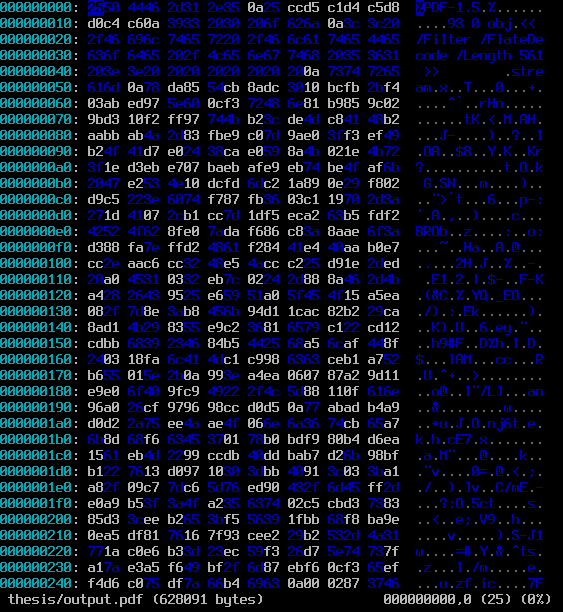
\includegraphics[scale=0.5]{static/be.png}
\caption{BHE: Binary Hex Editor}
\label{be}
\end{figure}

\pagebreak
\subsection{Υλοποίηση του Bitshred}
Η γλώσσα προγραμματισμού η οποία χρησιμοποιήθηκε για την υλοποίηση του Bitshred είναι η \emph{python}.
Η ευκολία χρήσης της συγκεκριμένης γλώσσας προγραμματισμού και η πληθώρα βιβλιοθηκών που υπάρχουν  είναι η αιτία που χρησιμοποιήθηκε.

Αρχικά, για τον διαχωρισμό του εκτελέσιμου κώδικα σε binary μορφή χρησιμοποιούμε την βασική βιβλιοθήκη της python και το πρόγραμμα \emph{readelf} από τα binutils για να ανοίξουμε το αρχείο και να βρούμε τα κομμάτια (sections) του εκτελέσιμου κώδικα.
\begin{lstlisting}[
    basicstyle=\ttfamily\footnotesize,
    frame=tb
]
f = open(file, "rb")
x_seg = os.popen("readelf -SW " + str(file) + " | grep AX", "r")
\end{lstlisting}

Στην συνέχεια αποκτώντας τα κομμάτια του binary τα χωρίζουμε σε chunks:
\begin{lstlisting}[
    basicstyle=\ttfamily\footnotesize,
    frame=tb
]
for off, size in segment.items():
    f.seek(int(off, 16))
    chunk = f.read(int(size, 16))
    exec_str += chunk.hex()
\end{lstlisting}

Έπειτα κάθε ένα από τα chunks τα εισάγουμε στον bloomfilter περνώντας τα από την hash function η οποία θα πρεπεί να είναι γρήγορη και αποδοτική.
Για αυτό τον λόγο χρησιμοποιούμε την \emph{MurmurHash3} η οποία είναι κατάλληλη για το σενάριο μας δηλαδή για \emph{hash-based lookups}.

\begin{lstlisting}[
    basicstyle=\ttfamily\footnotesize,
    frame=tb
]
bloom = BloomFilter(BLOOMSIZE, HASHCOUNT)
for vv in shreds:
    bloom.add(vv)
\end{lstlisting}

Τα δύο ορίσματα που παίρνει η BloomFilter είναι το μέγεθος του υποκείμενου bitarray \emph{BLOOMSIZE} και οι φορές που θα κατακερματιστεί το shred \emph{HASHCOUNT}.

Για να βρούμε τις αποδοτικές τιμές των ορισμάτων πρέπει να λάβουμε υπόψη τα εξής:

\textbf{Πιθανότητα Λανθασμένης Θετικότητας}: m είναι το μέγεθος του πίνακα bit, k είναι ο αριθμός των συναρτήσεων κατακερματισμού και n είναι ο αριθμός των αναμενόμενων στοιχείων που θα εισαχθούν στο φίλτρο, τότε η πιθανότητα ψευδώς θετικού p μπορεί να υπολογιστεί ως:

{\large$P=\left ( 1-\left [ 1- \frac {1}{m} \right ]^{kn} \right )$}

\textbf{Μέγεθος της σειράς Bit}:  n είναι γνωστός και η επιθυμητή ψευδής θετική πιθανότητα είναι p, τότε το μέγεθος της διάταξης bit m μπορεί να υπολογιστεί ως:

{\large $m = -\frac {n \ ln P} {(ln 2) ^ 2}$}
 
\textbf{Βέλτιστος αριθμός συναρτήσεων κατακερματισμού}: Ο αριθμός συναρτήσεων κατακερματισμού k πρέπει να είναι θετικός ακέραιος. Εάν το m είναι το μέγεθος bitarray και το n είναι ο αριθμός των προς εισαγωγή στοιχείων, τότε το k μπορεί να υπολογιστεί ως:

{\large $k = \frac {m} {n} ln 2$}

Αφού βρήκαμε τις βέλτιστες τιμές για το μέγεθος του bitarray και τον αριθμό συναρτήσεων κατακερματισμού προχωράμε στο επόμενο στάδιο δηλαδή στον υπολογισμό του δείκτη \emph{jaccard}.

\noindent Από το paper παίρνουμε τον τύπο του \emph{jaccard index}:

$J(A, B) = \displaystyle \frac{|A\space\cap B|}{|A\space\cup B|}$}\space\space\Rightarrow\space\space
$J(A, B) = \displaystyle \frac{F_{11}}{F_{01} + F_{10} + F_{11}}$}

\noindent Και τον μετατρέπουμε σε κώδικα:
\hspace{4pt}

\begin{lstlisting}[
    basicstyle=\ttfamily\footnotesize,
    ]
  def calc_jaccard(A, B):
    and_score = 0
    or_score = 0
    for a, b in zip(A, B):
        and_score += a & b  # F11
        or_score += a | b  # F01 + F10 + F11

    jaccard = and_score / or_score

\end{lstlisting}

Και έτσι με αυτό τον τρόπο καταλήγουμε σε ένα αποτέλεσμα το οποίο εκφράζει το ποσοστό ομοιότητας του εκτελέσιμου κομματιού των δύο προγραμμάτων.

Σε αυτό το σημείο θα γινόταν η παρουσίαση των δύο άλλων τεχνικών υλοποιήσεων των paper αλλά λόγω του περιορισμένου χρονικού πλαισίου της πτυχιακής εργασίας και του βαθμού δυσκολίας δεν έφτασαν σε ένα ικανοποιητικό και ολοκληρωμένο στάδιο.
